
%%%%%%%%%%%%%%%%%%%%%%%%%%%%%%%%%%%%%%%%%
% Short Sectioned Assignment
% LaTeX Template
% Version 1.0 (5/5/12)
%
% This template has been downloaded from:
% http://www.LaTeXTemplates.com
%
% Original author:
% Frits Wenneker (http://www.howtotex.com)
%
% License:
% CC BY-NC-SA 3.0 (http://creativecommons.org/licenses/by-nc-sa/3.0/)
%
%%%%%%%%%%%%%%%%%%%%%%%%%%%%%%%%%%%%%%%%%

\documentclass[paper=a4, fontsize=11pt]{scrartcl}
\usepackage[utf8]{inputenc}
\usepackage[spanish]{babel}
\usepackage{amsmath,amsfonts,amsthm}
\usepackage{sectsty}
\usepackage{fancyhdr}
\usepackage{sectsty}
\usepackage{graphicx}

\allsectionsfont{\textbf \normalfont}
\setlength\parindent{0pt}
\pagestyle{fancyplain}
\fancyhead{}
\fancyfoot[L]{Electrónica de Microondas}
\fancyfoot[C]{}
\fancyfoot[R]{\thepage}\fancyfoot[C]{}

\renewcommand{\headrulewidth}{0pt}
\renewcommand{\footrulewidth}{0pt}
\setlength{\headheight}{13.6pt}
\newcommand{\horrule}[1]{\rule{\linewidth}{#1}}
\newcommand{\exercisetitle}[1]{
\section{}
#1 \\[0.1cm]
\horrule{1pt}
}
\title{
\normalfont \normalsize
\huge Ejercicios Tema 3 \\
\horrule{2pt} \\[0.5cm]
}
\author{Luis Sánchez Velasco}
\date{\normalsize\today}

\begin{document}

\maketitle

\newcommand{\propconstant}[1]{
  \begin{equation*}
      \gamma = \sqrt{(R + j\omega L)(G + j \omega C)} #1
  \end{equation*}
}

\newcommand{\propconstantnoloss}[1]{
  \begin{equation*}
      \gamma =j\omega \sqrt{ L C} #1
  \end{equation*}
}

\newcommand{\impedance}[1]{
  \begin{equation*}
      Z_0 = \sqrt{\frac{(R + j\omega L)}{(G + j \omega C)}}  #1
  \end{equation*}
}

\newcommand{\impedancenoloss}[1]{
  \begin{equation*}
    Z_0 = \sqrt{\frac{L}{C}} #1
  \end{equation*}
}

\newcommand{\swr}[1]{
  \begin{equation*}
    SWR = \frac{1 + | \Gamma_L |}{1 - | \Gamma_L |} #1
  \end{equation*}

}

\exercisetitle{
Una línea de transmisión posee los siguientes parámetros por unidad de longitud: $L=0.3\mu H/m$, $C=450pF/m$,
$R=5\Omega /m$, y $G=0.01S/m$. Calcular la constante de propagación y la impedancia característica de esta
línea a $880MHz$. Recalcular estos parámetros en ausencia de pérdidas.}

La constante de propagación en medios con perdidas se define como:
\propconstant{ = \alpha + j \beta}
Donde sustituyendo por los valores dados en el ejercicio, $L=0.3\mu H/m$, $C=450pF/m$, $R=5\ohm /m$, y $G=0.01S/m$ obtenemos:
\begin{align*}
  \alpha &= 0.226 \\
    \beta &= 64.2
\end{align*}
Y para el cálculo de la impedancia característica:
\impedance{= 25.8 + 0.01j }
\\[0.5cm]
Para el caso sin perdidas asumiremos $R = G= 0$, por lo que la constante de propagación quedará como:
\propconstantnoloss{ = 64j}
y la impedancia característica:
\impedancenoloss{= 25.8 \Omega}

\exercisetitle{
Una línea de transmisión sin perdidas de longitud $0.3\lambda$ termina en una impedancia de carga, $Z_L$. Encontrar
el coeficiente de reflexión en la carga, el SWR de la linea y la impedancia de entrada de la linea. $(Z_0=75
\Omega, Z_L = 40 + j20 \Omega)$.
}
Para calcular primeramente el coeficiente de reflexión, situaremos en la carta de Smith el punto $z = \frac{40}{75} + \frac{20}{75}j \Omega$, marcado con un '1' en al gráfica. Donde observando el ángulo y la fase de este punto, obtenemos:
\[ \Gamma_L = 0.34e^{j2.45} \]

Para calcular el SWR haremos:
\swr{ \approx 2}

Para calcular la impedancia a la entrada moveremos el punto '1' $0.3 \lambda$ hacia el generador, punto '2' y observaremos que lineas corta. En este caso:
$z_i = 0.94 + 0.7i$ que al denormalizar quedará como: $Z_{in} = 67.5 + 52.5j$.

\begin{figure}[h]
  \centering
  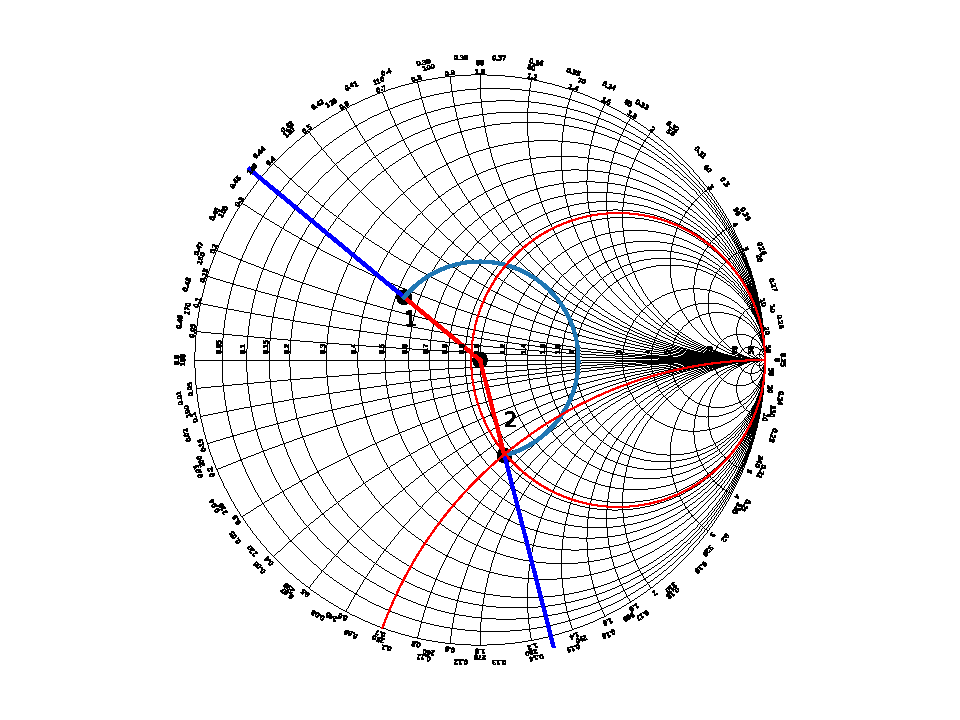
\includegraphics[scale = 0.85]{ej2/images/out.pdf}
  \caption{Moviendo el punto $0.3 \lambda$}
  \label{ej2smith}
\end{figure}

\exercisetitle{
Una línea de transmisión sin pérdidas de impedancia característica $Z_0$ se termina con una impedancia de
carga de $150 \Omega$.  Si se mide una SWR en la línea de 1.6, encontrar los dos posibles valores para $Z_0$.
}
Aunque el enunciado nos dice que existen dos posible valor para $Z_0$, solo existe uno, ya que tanto la impedancia de carga, como la de la línea (sin pérdidas), son reales.
Para resolverlo empezaremos evaluando la expresión del SWR:
\swr{ = 1.6}
Donde podemos resolver para $| \Gamma_L |$,obteniendo:
\[ | \Gamma_L | = 0.23 \]
Sabemos que al ser las dos impedancias puramente reales, el valor absoluto del coeficiente de reflexión será igual a su valor real, esto se puede observar en la expresión del coeficiente de reflexión en función de la impedancia de carga y la impedancia carcterística de la línea.

\reflectionfromimpedance{ = 0.23}

De donde podemos obtener $Z_0$, el cual resulta:
\[Z_0 = 93.9 \Omega \]

\exercisetitle{
Un transmisor wireless está conectado a una antena con impedancia de entrada de $80+j50\Omega$ a través de
un cable de $50\Omega$.  Si el transmisor de $50\Omega$ puede suministrar una potencia de 30W cuando se conecta a
una carga adaptada, ¿cuál es la potencia suministrada a la antena?  Repetir el cálculo suponiendo que el
transmisor tiene una impedancia de salida de $60\Omega$.
}

Nos encontramos on la situación en la que tenenemos una línea por la que circulan 30W, de los cuales el $100\%$ irán hacia la carga cuando esta este adaptada. Calcularemos que potencia irá hacia la carga en los siguientes casos:
\subsection{$Z_0 = 50\Omega$}
En este caso el coeficiente de reflexión será:
\reflectionfromimpedance{ = \frac{80+j50\Omega - 50\Omega}{80+j50\Omega + 50\Omega} = 0.418e^{j0.663} }
Y la potencia entregada:
\begin{align*}
  P_{in} &= P_{out}(1- \Gamma_L)
  P_{in} &= 30(1- 0.41)
  P_{in} &= 17.7 W
\end{align*}
\subsection{$Z_0 = 60\Omega$}
Repitiendo las cuentas:
\reflectionfromimpedance{ = \frac{80+j50\Omega - 60\Omega}{80+j50\Omega + 60\Omega} = 0.368e^{j1.533} }
Y la potencia entregada:
\begin{align*}
  P_{in} &= P_{out}(1- \Gamma_L)
  P_{in} &= 30(1- 0.368)
  P_{in} &= 18.96 W
\end{align*}

\exercisetitle{
Asumiendo que la impedancia característica es real, mostrar que para una carga puramente reactiva de
la forma $Z_L = jX_L$, la magnitud del coeficiente de reflexión es siempre la unidad.
}

Para demostrar esto empezaremos colocando la expresión del coeficiente de reflexión:
\[\Gamma_L = \frac{jX_L - Zo}{jX_L + Zo} \]
Y convertiremos tanto el divisor como el denominador a modulo y fase:
\begin{align*}
  \Gamma_L &= \frac{\sqrt{(X_L)^2 +(-Zo)^2]}e^{jarctan(\frac{X_L}{-Z_0} )}  }{\sqrt{(X_L)^2 +(Zo)^2]}e^{jarctan(\frac{X_L}{Z_0} )}  } \\
  \Gamma_L &= 1e^{j(\arctan{\frac{X_L}{-Z_0} } - \arctan{\frac{X_L}{Z_0} })}
\end{align*}
Como la función arcotangente es impar:
\[ \Gamma_L &= e^{-j2\arctan{\frac{X_L}{Z_0} }

Se puede ver como ambos modulos serían iguales, dividiendose los dos a 1, esto tiene sentido ya que si la caraga fuese puramente reactiva, no debería consumir ningún tipo de enrergía, por tanto toda ha de ser rebotada hacia el generador.

\exercisetitle{
Para  el  circuito  mostrado,  encontrar  la  potencia  transmitida  a  la  carga  y  la  potencia  disipada  en  el
generador para una impedancia de carga $Z_L= 30 +j40\Omega$.  ¿Qué valor de la impedancia de carga permitirá una entrega maxima de potencia a la carga?  ¿Cuál es esta potencia?

}
\subsection{$Z_L = 30 + 40 \Omega$}
Procederemos de la siguiente manera:
\begin{enumerate}
  \item Calcularemos la impedancia normalizada de la carga
  \item Situaremos esta impedancia en la carta de smith, obteniendo $\Gamma_L$
  \item Moveremos la línea $0.7\lambda$ hacia el generador para obtener $z_{in}$
  \item Denormalizaremos $z_{in}$ y obtenedremos la potencia entregada a la línea.
\end{enumerate}

\begin{figure}[h]
  \centering
  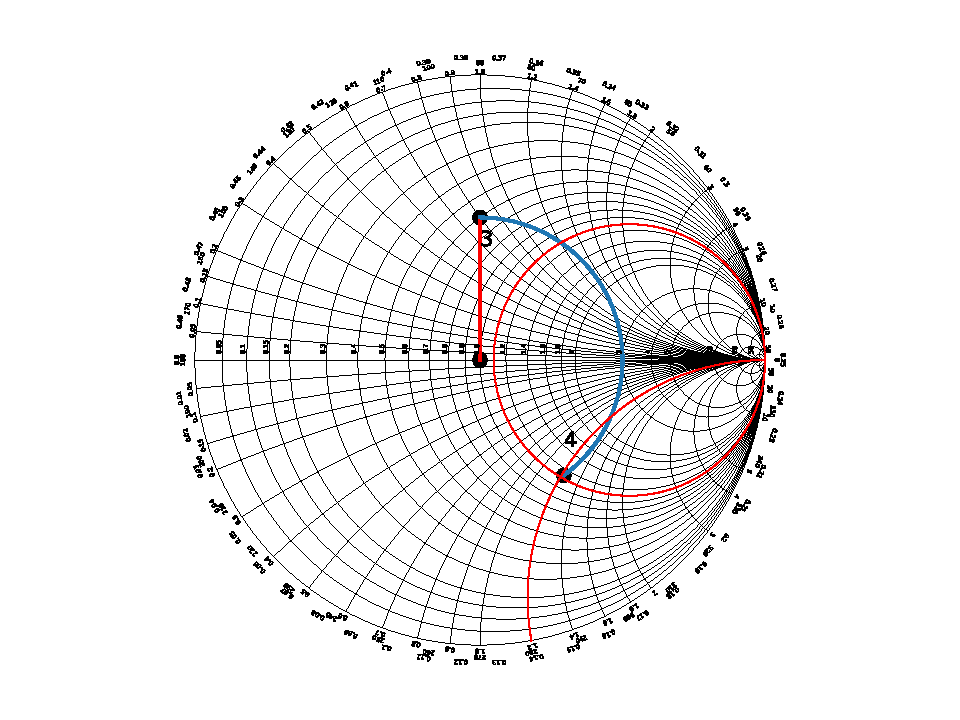
\includegraphics[scale = 0.85]{ej6/images/out1.pdf}
  \caption{Pasos 3 y 4}
  \label{ej2smith}
\end{figure}

En este caso $z_in = \frac{3}{5} + j\frac{4}{5}$, obteniendo, como se puede ver en la figura 2:
\[ \Gamma_L = 0.5e^{j1.57} \]
Tras mover la línea $0.7\lambda$ obtenemos $z_{in} = 1.1 + 1.2j$, que denormalizado queda como:
\[Z_{in} = 55 + 60j\]
 Con lo que podremos calcular la potencia de entrada a la línea con la siguiente expresión:
\begin{align*}
  P_{in} &= \frac{1}{2}|V_S|^2 \frac{R_{in}}{(R_S + R_{in} )^2 + (X_S + X_{in})^2}
  P_{in} &= \frac{1}{2}100  \frac{55}{(20+55)^2 + (30+60)^2}
  P_{in} &= 0.2 W
\end{align*}

Por lo tanto se entregarán 0.2W a la carga, ya que al no tener la línea perdidas, toda este energía se entregará a la carga.

\subsection{¿Qué valor de la impedancia de carga permitirá una entrega maxima de potencia a la carga?}
El valor que hará que esta potencia entregada a la carga sea máxima será el que haga que la impedancia de entrada a la línea sea: $Z_{in} = R_S - X_S$, por que empezaremos normalizando este valor con la impedancia del generador: $z_{in} = 0.4 + 0.6j$. Situaremos este valor en la carta de smith, y retrocederemos hasta la carga $0.7\lambda$, y la impedancia obtenida será la que máximize la potencia entregada  la carga.

\begin{figure}[h]
  \centering
  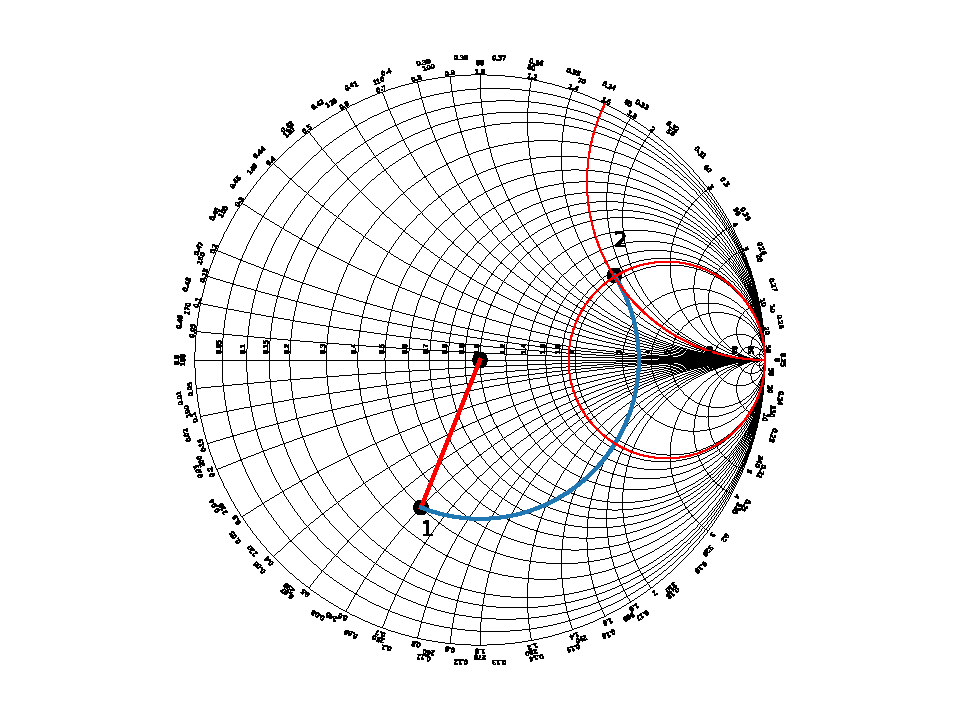
\includegraphics{ej6/images/out2.pdf}
  \caption{Avanzando $0.7\lambda$ hacia la carga}
  \label{ej2smith}
\end{figure}

Donde podemos ver que la impedancia normalizada $z_l = 1.9 +1.6j$, que denormalizada es $Z_L = 95 + 80j \Omega$

\subsection{¿Cuál es esta potencia?}
Podemos usar la expresión de la potencia entregada a la carga cuando la línea esta completamente adaptada a la línea:
\[P_{in} = \frac{|V_s|^2}{8R_s} = 0.625W\]

\exercisetitle{
En el circuito de la figura, usar la carta de Smith para encontrar el SWR de la línea, el coeficiente de reflexión en la carga, la admitancia de carga, la impedancia de entrada de la línea, la distancia desde la carga hasta el primer mínimo de voltaje, y la distancia desde la carga al primer máximo de voltaje.
}
Primero normalizaremos la impedancia en la carga como: $z_l = 1.4 + 0.8j$
\subsection{SWR y $\Gamma$}
Para calcular estos valores usando la carta de smith situamos la impedancia normalizada en la carta y medimos la distancia hasta el origen (0, 0),  usando las diferentes escalas en la parte de abajo podremos obtener los valores.
Estos valores resulta SWR = 2 y $\Gamma = 0.32$
\begin{figure}[h]
  \centering
  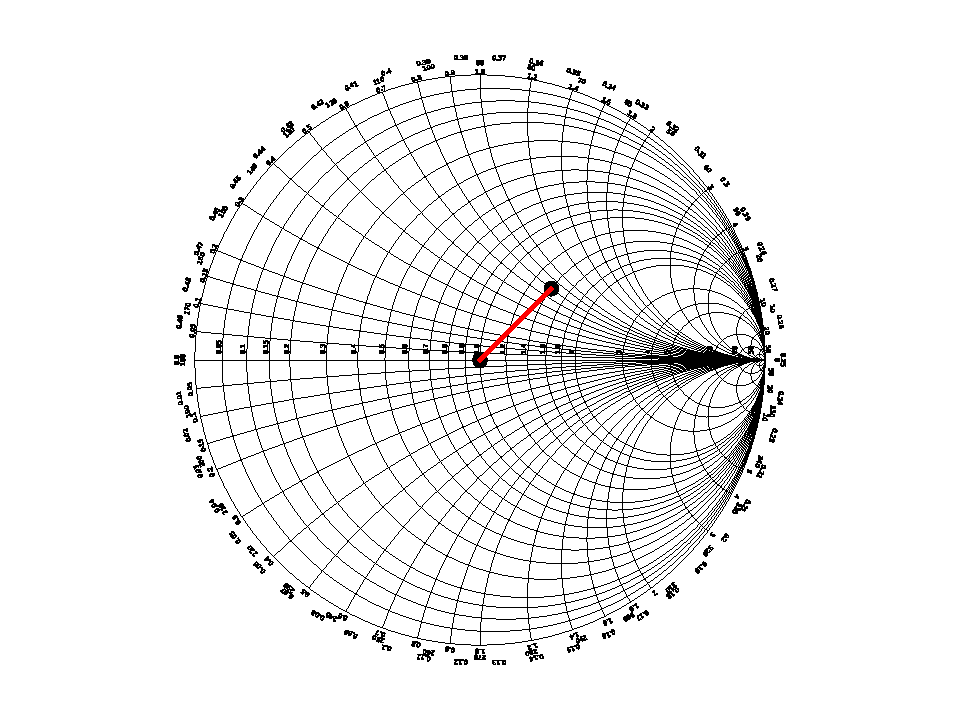
\includegraphics{ej7/images/out1.pdf}
  \caption{SWR y $\Gamma$}
  \label{ej2smith}
\end{figure}
\newpage
\subsection{Admitancia de la carga}
Para calcular la admitancia moveremos el punto anteriormente obtenido $180\º$ y denormalizaremos el mismo multiplicando por $\frac{1}{Y_0}$
\begin{figure}[h]
  \centering
  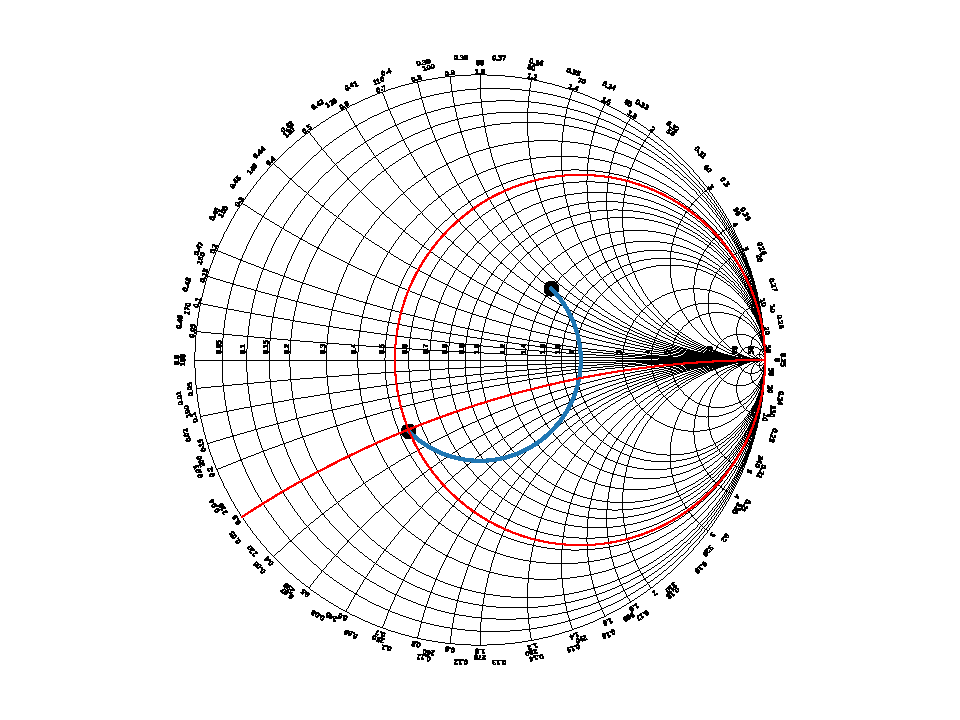
\includegraphics{ej7/images/out2.pdf}
  \caption{Admitancia}
  \label{ej2smith}
\end{figure}
\newline
Donde al denormalizar obtenemos $Y_l =  0.018 + j6 \times 10^{-3} S$
\newpage

\subsection{Impedancia de entrada}
Para hayar la impedancia de entrada simplemente moveremos el punto obtenido en primer apartado $0.8\lambda$ hacia el generado y denormalizaremos la impedancia

\begin{figure}[h]
  \centering
  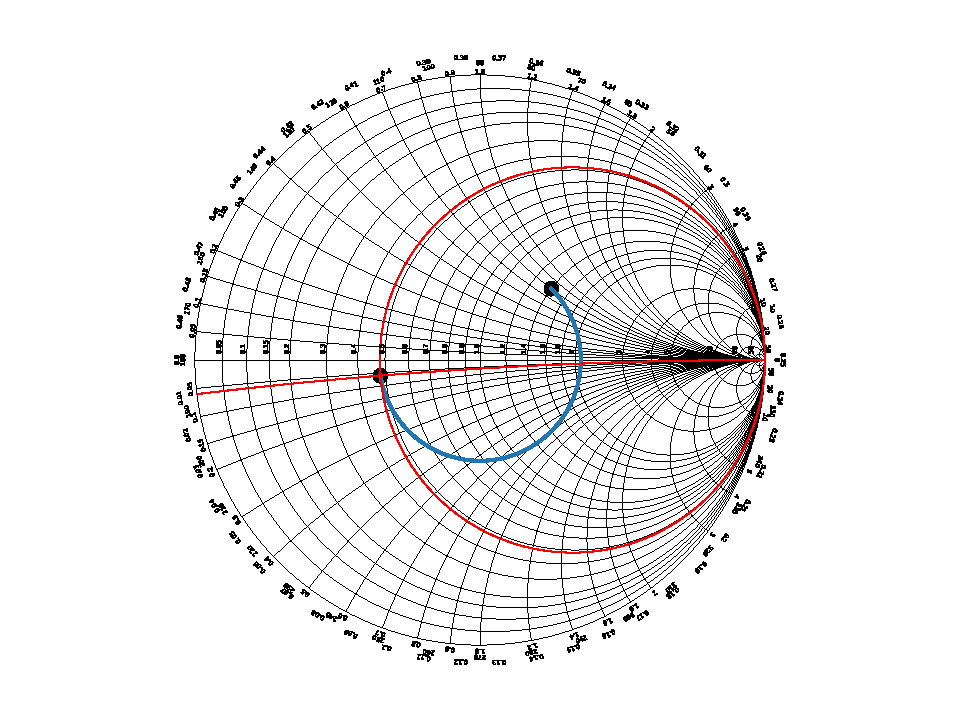
\includegraphics{ej7/images/out3.pdf}
  \caption{Impedancia de entrada}
  \label{ej2smith}
\end{figure}
Al denormalizar obtenemos $Z_{in} = 24 + 3j \Omega$
\newpage

\subsection{Máximo y mínimo}
Para hayar la distancia del primer máximo/mínimo nos fijaremos en el detalle de que los máximos y mínimos en la línea se producen cuando $Z(-l)$ es un número puramente real, por lo tanto la estrategia que seguiremos para hayar dichos puntos será avanzar el punto calculado en el apartado 1 hasta que la parte imaginaria sea 0, el siguiente máximo/minimo se encotrará a $\lambda / 4$ de este punto.
\begin{figure}[h]
  \centering
  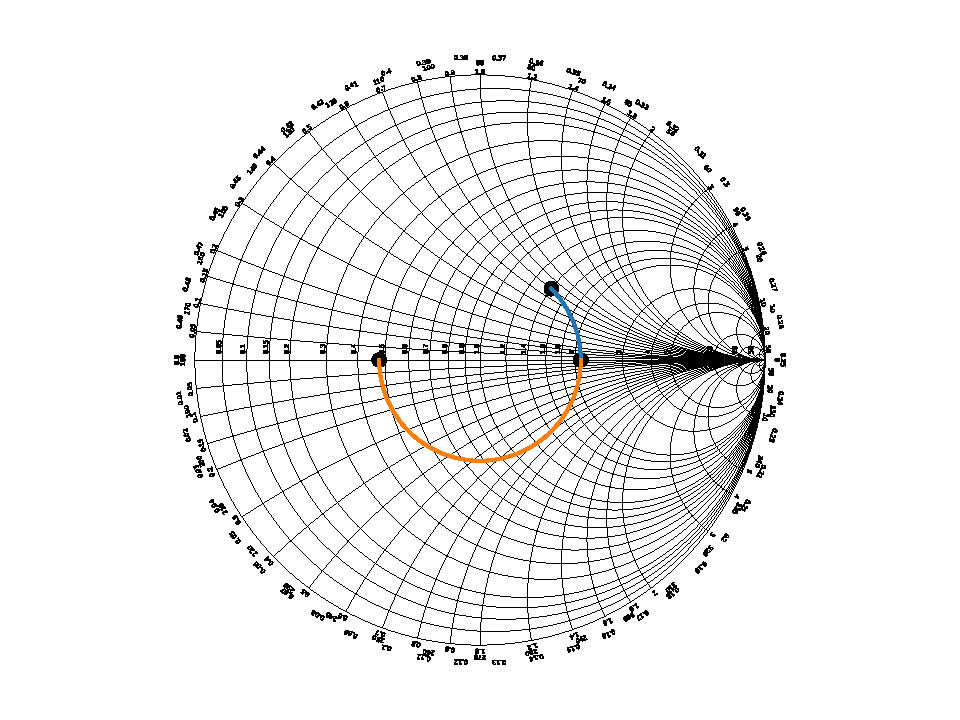
\includegraphics{ej7/images/out4.pdf}
  \caption{Máximo y mínimo}
  \label{ej2smith}
\end{figure}
Donde vemos que la distancia, en longitudes de onda, hasta el primer máximo ($Z_0 \leq Z(-l)$ ) es de $0.028\lambda$, por lo que el mínimo se encontrará a $0.278\lambda$.

\exercisetitle{
Una impedancia de carga de $Z_L=60+j30 \Omega$ se quiere adaptar a una línea de $50\Omega$ usando una longitud $l$ de una línea sin pérdidas con una impedancia característica $Z_I$. Encontrar los valores requeridos para $Z_I$ y $l$.
}

Resolveremos este ejercicio de forma analítica, debido a su complejidad usando la carta de smith (o al menos a mi no se me ocurre nada).
Usaremos la expresión que relacion la impedancia de entrada ($Z_{in}$) con la impedancia característica de la línea, la impedancia de carga y la longitud de la línea.
\[Z_{in} = Z_0 \frac{Z_L + jZ_0 \tan{ \beta l} }{Z_0 + jZ_L \tan{ \beta l} } \]
Que sustiyendo: (Queremos que $Z_in = 50 \Omega$ para que la línea esta adapatada)
\[50 = Z_0 \frac{60+j30  + jZ_0 \tan{ \beta l} }{Z_0 + j(60+j30 ) \tan{ \beta l} } \]
Que separando la parte real de la imaginaria en dos ecuaciones distintas:
\begin{align}
  3000 \tan{ \beta l} &= Z_0 + Z_0^2 \tan{ \beta l} \\
  -150 \tan{ \beta l} &= Z_0
\end{align}
Sustituyendo $\tan{ \beta l}$ de la ecuación (2) en la ecuación (1):
\begin{align*}
  50 Z_0 &= \frac{Z_0^2}{150}
\end{align*}
Donde obtenemos 3 soluciones $Z_0 = +86.6, -86.6, 0 \Omega$, donde podemos ver que la única con sentido físico es $86.8 \Omega$. Con este dato podemos vover a la ecución 2 para hayar la longitud de la línea:

\[-150 \tan{ \beta l} = 86.6 \]

Cuya solución es $\beta l = 0.52$, que dividiremos entre $2 \pi$ para obtener la longitud en longitudes de onda.
\[l = 0.083 \lambda\]

\exercisetitle{
Una línea de transmisión con $Z_0=50 \Omega$ está cargada con una impedancia de $Z_L=50+j35 \Omega$. ¿A qu ́e distancia
de la carga debe colocarse una sección adaptadora en $\lambda/4$ para acoplar la línea a la carga?  ¿Cuál debe
ser el valor de la impedancia característica de la sección $\lambda/4$
}
Se nos pide introducir una línea $\lambda/4$ en el sistema anterior con el fin de adaptar la línea a la carga. Para ello primero debemos encontrar a que distancia de la carga la impedancia se hace puramente real, con lo que podremos aplicar la expresión de una línea  $\lambda/4$.
\begin{figure}[h]
  \centering
  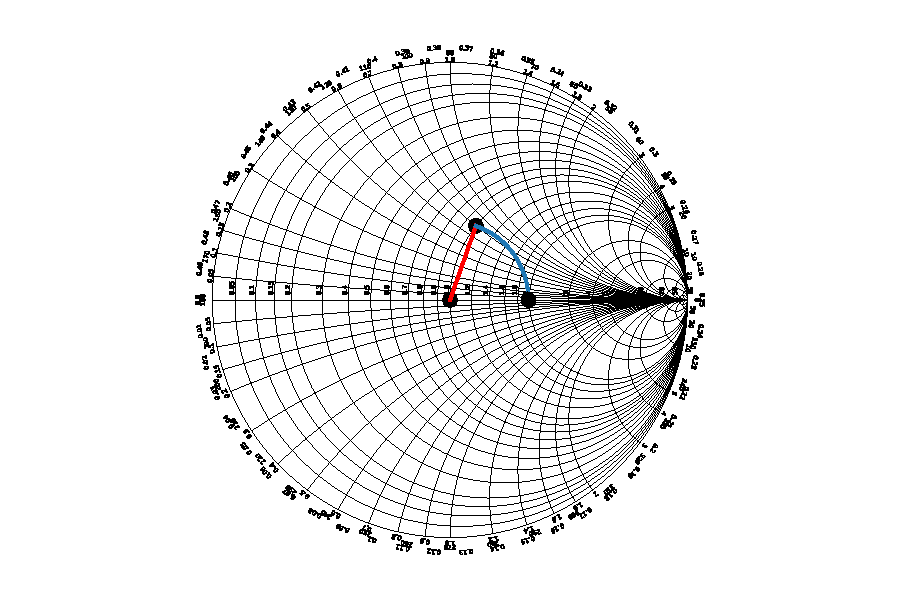
\includegraphics{ej9/images/out.pdf}
  \caption{$z_{in} = a + 0j$}
  \label{ej2smith}
\end{figure}

Donde vemos que $z_{in} = 2$ que tras denormalizar de $50 \Omega$, obtendremos $Z_{in} = 100 \Omega$, con esto ya podemos calcular la impedancia intrínseca de la insercción $\lambda/4$ como:
\[ Z_0 = \sqrt{Z_{in} Z_{Z_L}} = \sqrt{100 \times 50} = 70.7 \Omega \]

\exercisetitle{
En  el  circuito  de  la  figura,  alimentado  con  un  generador  de  alterna  con  amplitud 10V,  fase  nula,  e impedancia  de  generador  $50 \Omega$,  determine  la  potencia  media  disipada  por  la  impedancia  de  carga $Z_1$. Todas las líneas de transmisión tienen impedancia característica $Z_0=50 \Omega$.
}

Para realizar este ejercicio empezaremos calculando la impedanciade entrada al sistema completo.
\subsection{Rama $Z_1$}
La impedancia se encuentra en paralelo con un stub $0.08\lambda$, por lo que calcularemos la admitancia de ambos componentes y los sumaremos:

\begin{align*}
&  Y_{stub} &=& -j \frac{1}{Z_0 \tan{\beta l}} &=& -j0.0363 \Omega \\
&  Y_L && &=& 0.019 +3.8 4 \times 10^{-3} \Omega \\
&  Y_{A} &=& Y_{stub} + Y_L &=& 0.019 -j0.032\Omega \\
&  y_{a} &=& Y_{A} / Y_{0} &=& 0.96 -j1.62 \Omega
\end{align*}

Y ahora nos iremos a la carta de smith para mover la admitancia $\lambda$ hacia el generador
\begin{figure}[h]
  \centering
  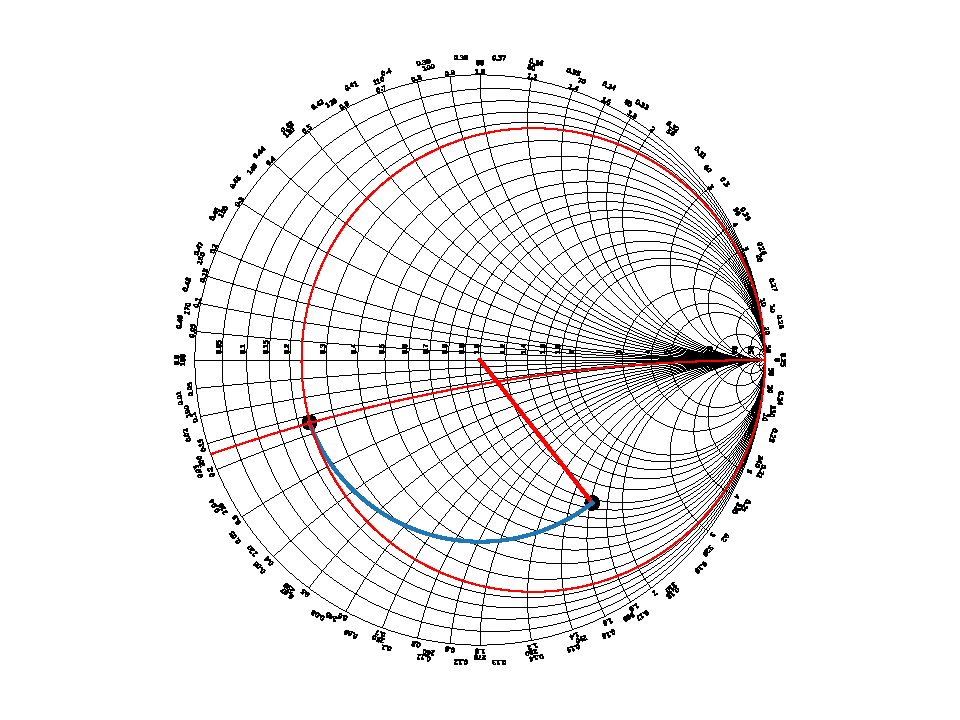
\includegraphics[scale = 0.75]{ej10/images/out1.pdf}
  \label{ej2smith}
\end{figure}

Donde comprobamos que la admitancia en ese punto para la rama $y_{r1} = 0.23 - 0.17j$. (Como todas las líneas tienen la misma impedancia característica, no tenemos porque denormalizar hasta el final)

\subsection{Rama $Z_2$}
Haremos lo mismo que se hizo en la anterior rama, pero podemos fijarnos en un detalla, la línea es de $0.25\lambda$, lo que significa que avanzaremos $\pi$ en la carta, si avanzamos otro $\pi$ para convertir a admitancia, daremos una vuelta completa, $2\pi$, por lo que podemos decir que la admitancia de entrada a la rama $Y_2$ es $5+j20 S$ que normalizado es $y_{r2} =0.1 + 0.4j$.

\subsection{Stub}
Primero necesitamos calcular la suma de las admitancias de las dos ramas, que resulta
$0.33 + 0.23j$, avanzaremos esta líneza $0.1\lambda$ y le sumaremos la admitancia delstub en paralelo, cuya admitancia normalizada es:
\[ y_{stub} = -j Z_0 \times \frac{1}{Z_0 \tan{\beta l}} = -j1.37 \]
Después avanzaremos la línea otros $0.15\lambda$ para obtener finalmente la admitancia de entrada. Estos movimientos se ven en la siguiente carta:
\begin{figure}[h]
  \centering
  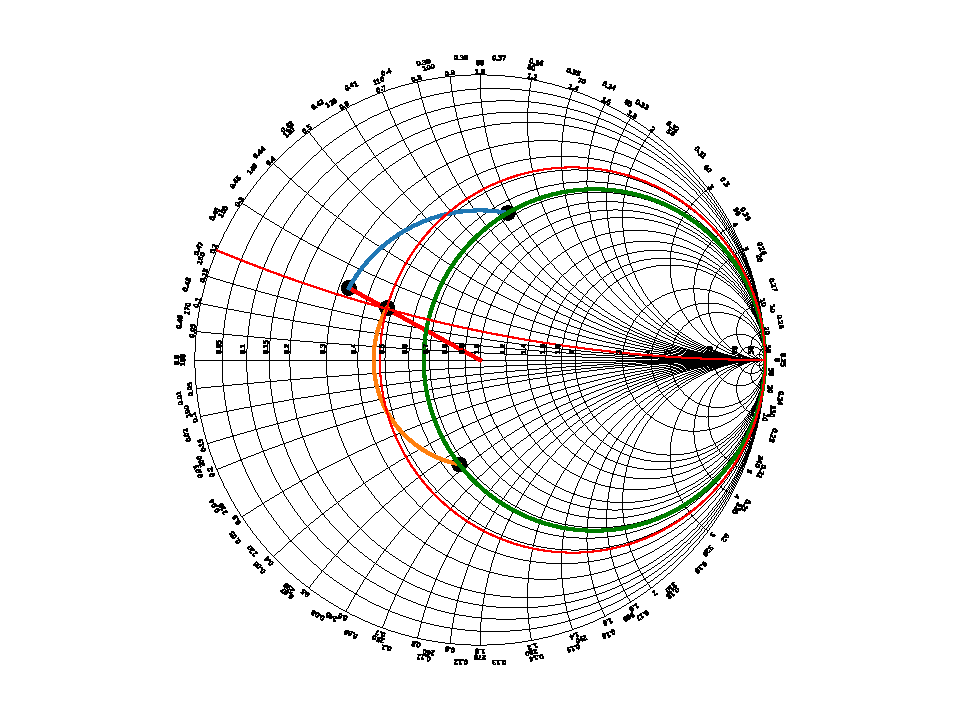
\includegraphics[scale = 0.75]{ej10/images/out2.pdf}
  \label{ej2smith}
\end{figure}
Donde podemos ver que al final obtenemos una admitancia de entrada de $y_{in} = 0.48 - j0.17$, que traducido a impedancia resulta $1.85 + j0.65$, que al denormalizar resulta:
\[Z_{in} =92.5 + j32\Omega \]

\subsection{Potencia entregada a $Z_1$}
Para ello, empezaremos calculando el voltaje de entrada:
\[V_{in} = V_S \frac{Z_{in}}{Z_S + Z_{in} } = 6.7e^{j0.114}\]
Este voltaje será el mismo a través de la línea, hasta que llegue hasta las ramas 1 y 2, ya que no hay perdidas, por tanto:
\begin{align*}
  P_{in} &= \frac{1}{2} |V_{in} |^2 \Re (\frac{1}{Z_{r1}^*})\\
  P_{in} &= \frac{1}{2} |V_{in} |^2 \Re ({Y_{r1}^*}) \\
  P_{in} &= 0.23 W
\end{align*}

\exercisetitle{
Determinar la potencia disipada por la impedancia de carga $Z_L$ en el circuito de la figura, donde todas las líneas de transmisión son sin pérdidas $(Z_{01}= 50\Omega ,Z_{02}=Z_{03}= 70\Omega ,Z_S= 20 +j30\Omega,Z_L= 25 +j10Ω)$. Modifique convenientemente $l_2$ y $l_3$ para alcanzar, si es posible, máxima transferencia de potencia.
}

La estrategia a seguir para resolver este porblema será la siguiente:
\begin{enumerate}
  \item Sabiendo que para conseguir la máxima potencia de transferencia necesitamos que $Z_in = Z_S^*$ moveremos $Z_in$ $0.2\lambda$ hacia la carga.
  \item Escogeremos una $l_3$ tal que la parte real sea igual a la parte real de la $Z_in$ movida hasta dicho punto.
  \item Escogeremos $l_2$ de forma que la parte imaginaria de la admitancia de la suma de la sección $l_3$ más el stub sean igual a la encontrada en el primer paso.
\end{enumerate}

\begin{figure}[h]
  \centering
  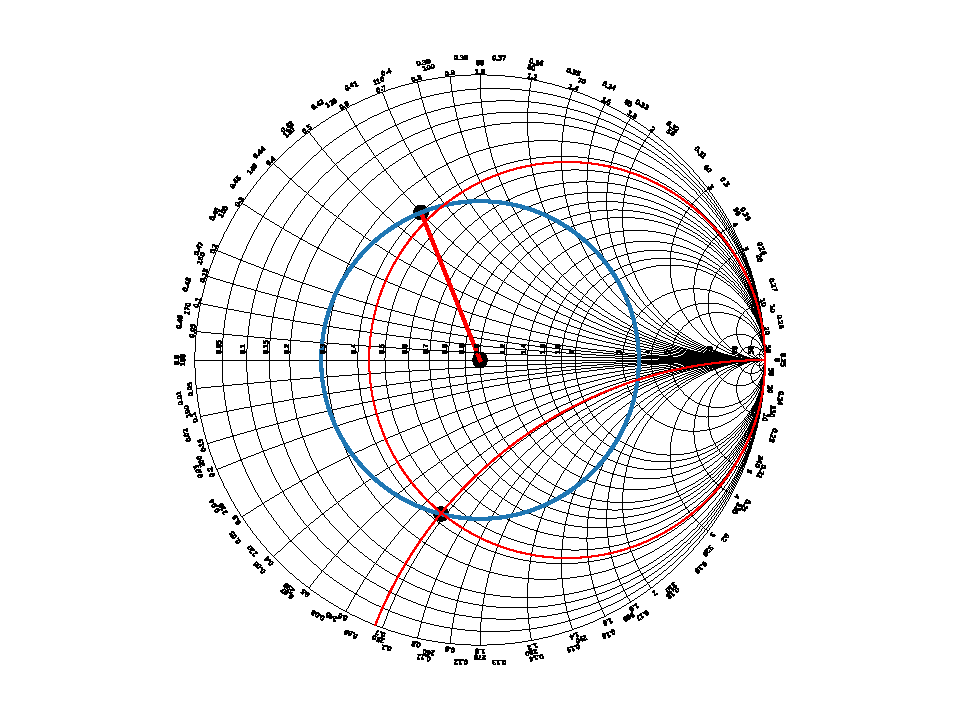
\includegraphics[scale = 0.75]{ej11/images/out1.pdf}
  \label{ej2smith}
\end{figure}
Obtenemos al final los valores normalizados $0.44 + 0.68j$ que al denormalizar y convertir en admitancia, obtendremos $y = 0.0134 -j0.02$

\subsection{$l_3$}
Para obtener la longitud $l_3$, nos moveremos por la línea, partiendo desde $y_l = 1/z_l= 2.62 -1.14 $, hasta encontrar una parte real de la admitancia igual a $0.0134$, que normalizado a la línea de $70 \Omega$ es $0.93$

\begin{figure}[h]
  \centering
  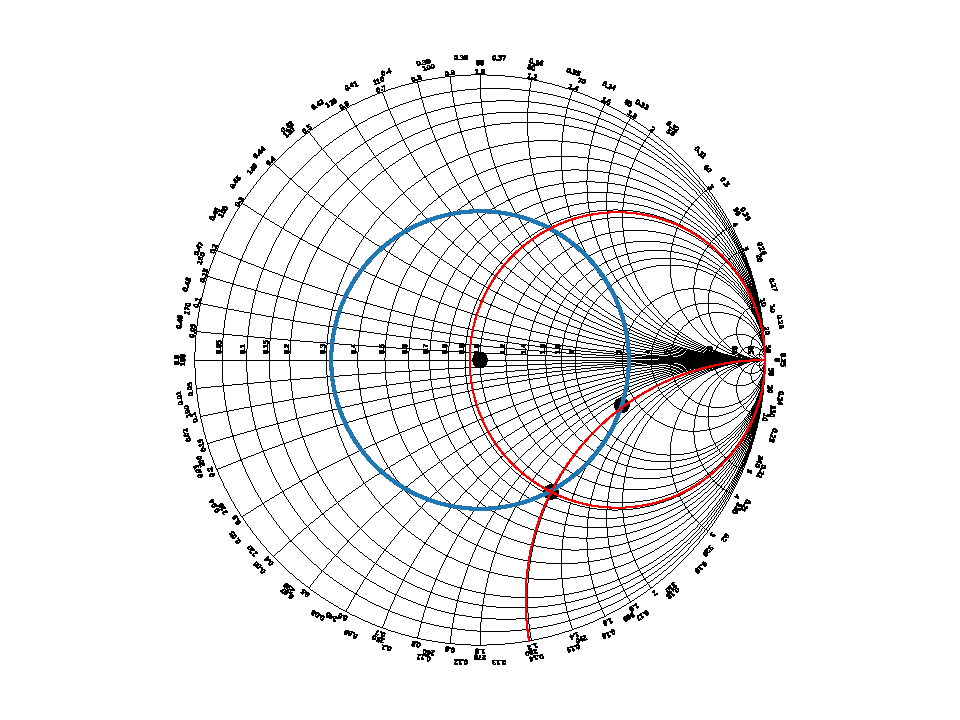
\includegraphics[scale = 0.75]{ej11/images/out2.pdf}
  \label{ej2smith}
\end{figure}

Donde vemos que esta la longitud de la línea ha de ser $0.1225\lambda$.

\subsection{$l_2$}
Como vemos la parte imaginaria de la admitancia de la línea $Z_L$ resultó ser -1.19, por lo que necesitamos un stub que nos situe la parte imaginaria en -0.02, por lo que de acuerdo con la ecuación (teniendo en cuenta que los valores estan normalizados):
\[y_{stub} = -j \frac{1}{tan{\beta l}} \]

Donde obtenemos $\beta l =   0.168$


\end{document}
